
\chapter{Sensor}

[metre le détail des methodes ICA si pas assez de maths]

\section{CSP algorithm}

\subsection{CSP running time optimization}
\label{Sec:running_time_optimisation}

L'implémentation initiale naïve de l'algorithme des CSP mettait une journée entière calculer pour un seul subject. Il était donc crutial de trouver des manières d'acceler fortement les calculs, qui seront dès lors repetés à chaque commit de la pipeline dans le cadre de l'integration continue avec Circle CI.

Un grand effort de recherche et d'ingénieurie à alors été mené pour réduire le temps de calculs.

\subparagraph{Technique d'ingenieurie logicielles classique}

Les techiques d'ingénieuries logicielles classique ont été clefs pour accellerer massivement les temps de calculs : - factoriasation de toutes les étapes, utilisation des outils tels que le line-profiler, qui permet de visualiser le temps d'execution de chacune des lignes. D'aptres part, même si mathématiquement certaines opération son commutatives, en pratique, le choix de l'ordre des opératio permet d'économiser du temps de calcul : par exemple même si l'opération (time crop, frequency filter), il vaut mieux commencer par crop la donnée puis filtrer, car l'opération de filtrage est très couteuse.


\subparagraph{Reduction de la dimensionalité}

Une fois toutes les améliorations logicielles approtées, on peut egalement apporter des améliorations venant des techniques du machine learning en utilisant des techiniques de reduction de dimensionalité, soit en selectionnant le type de channels, soit en utilsnat une PCA:

\begin{figure}[ht]
    \centering
    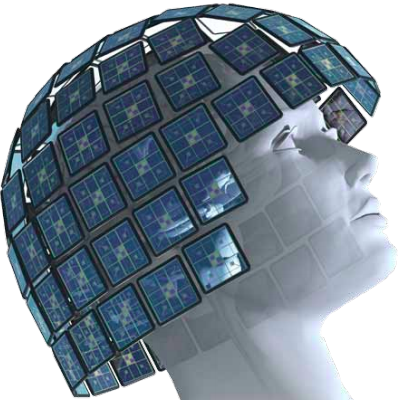
\includegraphics[width=5cm]{images_report/sensor/sensors_elekta.png}
    \caption[MEG Sensors [\href{https://www.elekta.com/dam/jcr:ed6d88e7-cd3e-478e-9c4a-3f89ef90ec92/Elekta-Neuromag-TRIUX-Brochure.pdf}{ELekta documentation}]]%
    {MEG Sensors [\href{https://www.elekta.com/dam/jcr:ed6d88e7-cd3e-478e-9c4a-3f89ef90ec92/Elekta-Neuromag-TRIUX-Brochure.pdf}{ELekta documentation}]}
    \label{sensors_elekta}
\end{figure}

\begin{itemize}
    \item Reduction de la dimensionalité par selection du type de channel: Les données MEG provient de sensor, qui sont au nombre de 102 et qui sont repartis comme sur la figure \ref{sensors_elekta}. Chaque sensor est constitué de 2 gradiometers mesurant le champs gradiometrique (Tesla/meter) suivant les directions tangente au plan du sensor, et d'un magnetometers mesurant le chanps electrique dans le suivant la normale au plan du sensor. Les magnetometres sont robustes au bruit exterieur tandis que les magnetometres sont davantages exposées. Mais les magnetometres ont deux avantages capitaux : 1. Ils enregistrent une information spatiale localisée, ce qui convient parfaitement à l'algorithme des CSP, qui qui favorise par la suite l'interpretabilités des patterns issus des CSP. 2. Les magnetometres sont deux fois moins nombreux que les gradiometres. AInsi, en selectionnant uniquement les magnetometres, on divise par trois le nombre de channells. L'algorithmes des CSP étant limité par une SVD dont la complexité en $\mathcal{O}(T n^2)$ évolue en fonction du carré de nombre $n$ de channels \cite{dhillonalan}, on accellère ainsi l'algorithme par un facteur 9. (T is the number of time point, in our case bigger than the number of channels. La complexité de la SVD interne au CSP est en carré du minimum entre $T$ et $n$).
    \item Le point presceent ne s'applique qu'à des données provenant d'une MEG, mais ne s'applique pas aux EEG. En effet, les EEG ne possèdent qu'un seul tyepe de channel. Il faut donc réduire la dimensionalité à l'aide d'une simple PCA.
\end{itemize}


\subparagraph{Sampling}

- CV, decimation, niquist

La dernière manière d'accellerer les temps de calculs est de faire du sampling sur 


\subparagraph{CSP running time optimization results}

Le choix de l'ordre de la commutativité, la reduction de la dimensionalité et le resampling nous permettent aujourd'hui d'obtenir des résultats en moins de trois heures avec 8Cross validation pour tous les sujects. C'est trois techniques permettent d'acceller respectivment par $2*10*5$ sur notre jeu de donnée tout en conservant des performances en tout point similaire. Il semblerait même que la PCA augmente la stabilité numérique des résultats.


% - Interaface avec le reste de la pipeline, openscience, reproductibilité
% - Anexes : Implémentation et choix d'architecte logiciel




\subsection{Iterations levels}

Choisir l'ordre des iterations n'a pas été une mince affaire, bien que ce soit ici plus un probleme d'ingénieurie que de la recherche pure.

- contrasts
- We iterate through subjects and sessions
- If there are multiple runs, runs are concatenated into one session.

\subsection{CSP Regularization}

\subsection{CSP : Variance vs Second order moment}

\subsection{CSP Solving}


\subsection{Subtilités mathématiques}

\paragraph{Why not aiming for the best classifier?}
Mathetically we do not seek here to create the best classifier,
and to optimize the rocauc score, we only seek
to obtain unbiased scores usable afterwards in the permutation test.
This is why it is not a big deal to optimize the running time
by making some approximations, such as:
- Decimation
- Selection of the mag channels, which contain a very large part of
the information contained in (mag+grad)
- PCA, which is very useful to reduce the dimension for eeg
where there is only one channel type.


\paragraph{philosophie de pourquoi c'est ok de réduire un peu les performances, Pourquoi ne pas se battre pour les performances avec les csp.}

By thinking more about it, It feels to me that this group cross validation is not even necessary at all for mathematical rigor. Because here we just want to construct a statistic for each frequency bin. Here our statistic is the size of the cluster after thresholding the roc auc score coming from a usual cross validation. But our statistic could really be anything. The permutation test is just here to confirm that "There is a difference", whatever the difference is. So it's perfectly valid to use any metric : accuracy is as legitimate as roc auc and our cross validation is as legitimate as a group cross validation.
Another way to say it is that : we do not want to test the generalization ability of our classifier between different runs. We just want to say : Our classifier proves a difference exists between the two conditions.
So I think no need to worry because no need for group cross-validation.


\paragraph{Possiblité de mettre un des frequences et des crop non uniformes}




\section{Permutations statistics algorithm}

\subsection{t-values calculation}

Les t-valeur est un test parametrique qui suppose la gaussianité des valuer sours jacentes caluclé. Cette hypothése de gaussianité n'es past tojours vrifiée dpour des données venant d'imagerie cerebrale en raison des nombreux filtres préliminaires. Mais dans notre cas, on calucle les t-valeur à partir de la différence entre le roc-auc score et le niveau de chance moyen ce qui permet de rétablir l'hypothese de gaussianité.

Le calcul des p-valeurs se fait pour chaque time-frequency bin de manière indépendante.

On considère la liste des différences $(X_i)_{i \in [\text{Nb Subjects}]}$ pour tous les sujets entre le roc-auc et le chance level $c=0.5$ pour une time frequency bin.

On soustrait alors toutes ces cartes au chance level d'une roc-auc à savoir $0.5$. On obtient alors la différence entre le roc-auc et le chance level.

Il suffit alors de Calculate the T-test for the mean of ONE group of scores.

This is a test for the null hypothesis that the expected value (mean) of a sample of independent observations a is equal to the given population mean, popmean.

Ce test permet de rejeter l'hypothese nulle sous laquelle la moyenne d'une population d'observation independantes est egal à $0$.

Formellement,
On veut comparer la moyenne $\mu$ d'une population de loi normale et d’écart type $\sigma$ non connu à $0$. Pour ce faire, on calcule la moyenne empirique $\overline{x} = \frac{1}{n}\sum_{i=1}^{n}x_i$ et l'estimateur  sans biais $S^{\ast ^2}_n$ de sa variance $\sigma^2$
:$S^{\ast ^2}_n = \frac{1}{n-1}\sum\limits_{i=1}^n (X_i - \overline X_n )^2$.

Selon l’hypothese nulle, la distribution d’échantillonnage de cette moyenne se distribue elle aussi normalement avec un écart type $\frac{\sigma}{\sqrt{n}}$.

La statistique de test:

$ Z = \sqrt{n}\frac{\overline{X} - \mu_0}{S^{\ast}_n}$
suit alors une [[loi de Student]] à $n-1$ degrés de liberté sous l'hypothèse nulle (c'est le théorème de Cochran).

On choisit un risque $\alpha$, généralement $0.05$ ou $0.01$ et l'on calcule la réalisation de la statistique de test :

:$z = \sqrt{n}\frac{\overline{x}_n - \mu_0}{s^{\ast}_n},$ où $s^{\ast}_n =\sqrt{\frac{1}{n-1}\sum\limits_{i=1}^n (x_i - \overline x_n )^2} $

% Si l'on veut tester H0 : μ ≥ μ0 :
% Si z est inférieur au quantile d'ordre α de la loi de Student à n – 1 degrés de liberté alors on rejette l'hypothèse nulle.

% Implémentation se fait à l'aide la fonction scipy.stats.ttest_1samp.




\chapter{Source}